\section{Incremental Shortest Paths with Predictions}

This section gives the algorithm and analysis for the online version of the problem with predictions. Recall that in this model the edges arrive online.  The goal of the algorithm is to maintain an array $D$ of length $n$.  At any time $t$, $D[i]$ should contain a $(1 + \epsilon)$-approximation of $d^t(v_i)$.

\subsection{The Algorithm}
This section describes the online algorithm. Before any edges arrive, the algorithm is given a prediction $\hat{\sigma}$ of the edge arrival sequence.  

\paragraph{Updated Predictions.}
Our algorithm dynamically maintains the predicted sequence of edge inserts by changing $\hat{\sigma}$ online.  Specifically, after the $t$th edge arrival, the algorithm will construct a new prediction which we refer to as $\hat{\sigma}_t$.  Initially,  $\hat{\sigma}_0 = \hat{\sigma}$. We call the sequence  $\hat{\sigma}_t$ the \defn{updated prediction}. 
Intuitively, the algorithm modifies the updated prediction after each edge arrival based on which edge actually arrives. 
 
For each edge $e$, let $\widehat{\ind}_t(e)$ be the position of $e$ in $\pred_t$.  Let $\ind(e)$ denote the position of $e$ in $\sigma$ (i.e.\ the true time when $e$ arrives). If $e \notin \pred_t$, then we define $\widehat{\ind}_t(e) := m+1$. 

Our algorithm updates the sequence of edges to agree with all edges seen so far.  In other words, at time $t$, the algorithm maintains that for all edges $e$ that arrive by $t$ in $\sigma$, $\widehat{\ind}_{t}(e) = \ind(e)$.

\paragraph{Maintaining Metadata from the Offline Algorithm.}
Since the online algorithm continuously updates the result of the offline approach, it stores information to help it navigate the result of the offline algorithm.

Recall that the offline algorithm stores, for each time $t$, the set of vertices and edges alive at time $t$, as well as a distance estimate $\hat{d}^{t}(v)$ for any vertex $v$ alive at time $t$.  
The online algorithm maintains exactly the same information.  
We will see that the algorithm updates these estimates continuously as the updated prediction changes.

\paragraph{Algorithm Description.}

First, let us describe the preprocessing performed by the algorithm before any edges arrive.
The algorithm sets $D[i] = \infty$ for all $i$, except for $D[1] = 0$, which represents the source. 
Then, the algorithm runs the offline algorithm from Section~\ref{sec:offline} on $\hat{\sigma}$.   
By running the offline algorithm, the algorithm will store $\hat{d}^t(v)$ for all times $t$ and all nodes $v$ alive at time $t$.   

Now, let us describe how the algorithm runs after the $t$th edge is inserted.
At each time $t$, the algorithm \emph{rebuilds} a subset of all the subproblems.  These rebuilds update the precomputed $\hat{d}^t(v)$. When a subproblem is rebuilt, all of its descendants are rebuilt as well.  The rebuilding procedure is formally described below. 

Let $e_t$ be the edge that arrives at time $t$, and let $t'= \widehat{\ind}_{t-1}(e_t)$, i.e., $t'$ is the predicted arrival time for $e_t$ in the updated predictions immediately before it arrives. 
Note that since the first $t-1$ edges of $\sigma$ and $\pred_{t-1}$ are the same, we always have $t' \geq t$ (assuming the edges in the input sequence are distinct).

First, we describe how the algorithm updates $\hat{\sigma}_{t-1}$ to get $\hat{\sigma}_t$.
\begin{itemize}
    \item If $t = t'$, i.e., the position of $e_t$ is predicted correctly at the time it is seen, then set $\pred_t := \pred_{t-1}$.
    \item If $t \neq t'$ and $t' \leq m$; that is, $e_t$ is predicted to arrive at a later time. In this case, the algorithm moves $e_t$ from position $t'$ to position $t$ in $\hat{\sigma}_{t-1}$, and shifts everything between $t$ and $t'$ one slot to the right to obtain $\pred_t$. 
    \item If $t \neq t'$ and $t' = m + 1$; that is, at time $t-1$, $e_t$ is not in the predicted sequence.  In this case, the algorithm inserts $e_t$ in position $t$, shifts the rest of the sequence one slot to the right, and truncates the predicted sequence to length $m$ to obtain $\pred_t$. 
\end{itemize}

\paragraph{Rebuilding Subproblems.} 
Next, the algorithm \defn{rebuilds} subproblems.  Recall that the algorithm given in Section~\ref{sec:offline} is recursive; each of its recursive calls can be represented by a node in the recursion tree. 

To rebuild a subproblem $[\ell, r]$, the offline algorithm is called on $[\ell, r]$ using the updated prediction $\hat{\sigma}_t$.  The rebuild makes recursive calls as normal.
Any time a subproblem with midpoint $x$ is rebuilt, the value of $\hat{d}^{x}(v)$ is updated based on the rebuild for all alive vertices $v$.  

Let $[\ell_m, r_m]$ be the largest subproblem with $t \leq (\ell_m+r_m)/2 < t'$; then the algorithm rebuilds $[\ell_m, r_m]$. As mentioned above, all descendants of $[\ell_m, r_m]$ will be recursively called, and therefore rebuilt as well.  
In other words, the algorithm rebuilds all the subproblems $[\ell, r]$, with $t \leq (\ell+r)/2 < t'$, and all of their descendants from top to bottom (so in the first case, no subproblem gets rebuilt). 
See Figure~\ref{fig:tree_jump} for an illustration. 
Let $\rebuild(t)$ be the set of all times $t''$ such that $t''\in [\ell, r]$ for some $[\ell, r]$ rebuilt at time $t$. If no subproblem is rebuilt at time $t$, we define $\rebuild(t) := \{t\}$ to insure that $t$ is always in $\rebuild(t)$. 

\paragraph{Updating the Distance Array.}
Finally, the algorithm must update the array $D$ containing the estimated distance to each vertex. 
When a new edge is inserted, some of the entries in $D$ need to be overwritten, as their estimated distance might have changed. 
At each time $t$, we want to have $D[i] = \hat{d}^t(v_i)$ for all $i$. 
To do so, the algorithm does the following for each time $t' \in \rebuild(t)$, where $t' \leq t$, in sorted order. The algorithm iterates through all alive vertices $v_i$ in $G_{t'}$, and sets $D[i] = \hat{d}^{t'}(v_i)$. 

\begin{figure}
    \centering
    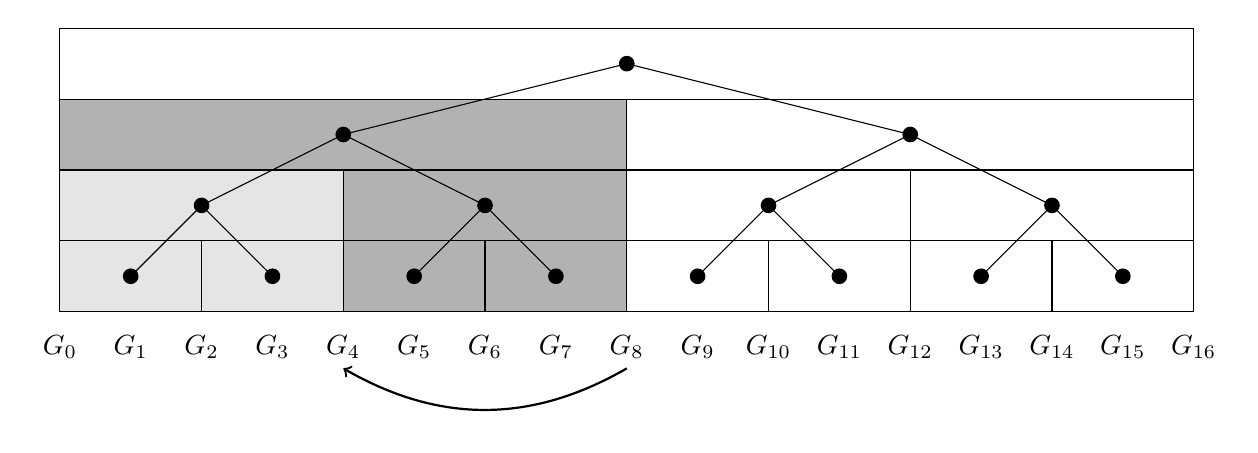
\begin{tikzpicture}[main/.style = {fill = black, circle, inner sep = 2pt}, 
    label/.style = {fill = none, circle, inner sep = 3pt},
    scale = 0.9]
        \draw[step = 1cm, gray, thin] (0,1) grid (16,5);
        \filldraw[fill = white, draw = black] (0,5) rectangle (16,4);
        \foreach \i in {0, 8}
            \filldraw[fill = white, draw = black] (\i,4) rectangle (\i+8,3); 
        \foreach \i in {0, 4, ..., 12}
            \filldraw[fill = white, draw = black] (\i,3) rectangle (\i+4,2);    
        \foreach \i in {0, 2, ..., 14}
            \filldraw[fill = white, draw = black] (\i,2) rectangle (\i+2,1);

        \foreach \i in {0, 1, 2, ..., 16}
            \node[label] at (\i, 0.5) {$G_{\i}$};    
   
        \draw[->, thick, black] (8,0.2) to [out = -150, in = -30] (4,0.2);
        \filldraw[fill = gray!60, draw = black] (0,4) rectangle (8,3);
        \filldraw[fill = gray!60, draw = black] (4,3) rectangle (8,2);
        \filldraw[fill = gray!60, draw = black] (4,2) rectangle (6,1);
        \filldraw[fill = gray!60, draw = black] (6,2) rectangle (8,1);

        \filldraw[fill = gray!20, draw = black] (0,3) rectangle (4,2);
        \filldraw[fill = gray!20, draw = black] (2,2) rectangle (4,1);
        \filldraw[fill = gray!20, draw = black] (0,2) rectangle (2,1);
        
        \node[main] at (8, 4.5) {};
        \foreach \i in {4, 12}
            \node[main] at (\i, 3.5) {};
        \foreach \i in {2, 6, 10, 14}
            \node[main] at (\i, 2.5) {};
        \foreach \i in {1, 3, ..., 16}
            \node[main] at (\i, 1.5) {};
    
        \foreach \i in {4, 12}
           \draw (8, 4.5) -- (\i, 3.5);
        \foreach \i in {2, 6}
           \draw (4, 3.5) -- (\i, 2.5);
        \foreach \i in {10, 14}
           \draw (12, 3.5) -- (\i, 2.5);
        \foreach \i in {1, 3}
           \draw (2, 2.5) -- (\i, 1.5);
        \foreach \i in {5, 7}
           \draw (6, 2.5) -- (\i, 1.5);
        \foreach \i in {9, 11}
           \draw (10, 2.5) -- (\i, 1.5);
        \foreach \i in {13, 15}
           \draw (14, 2.5) -- (\i, 1.5);  
    \end{tikzpicture}    
    \vspace{-.12in}
    \caption{An illustration of the subproblems that get rebuilt during one edge insertion. In this example, at time $t=4$, the edge $e_4$ was predicted to arrive but edge $e_8$ has arrived. So the algorithm moves edge $e_8$ from position $t'=8$ to position $t=4$. The algorithm then rebuilds all the subproblems with $t \leq (\ell+r)/2 < t'$ (colored dark gray) and their descendants (colored light gray) from top to bottom.}
    \label{fig:tree_jump}
    \vspace{-.03in}
\end{figure}

\subsection{Analysis}

This section establishes the theoretical guarantees of the algorithm. That is, the correctness of the approximation of the distances as well as the runtime bounds. 

We begin with some structure that applies to any run of the \emph{offline} algorithm.  This will help us argue correctness of our algorithm.
\begin{lemma}
\label{lem:dead_estimates_dont_change}
    For any sequence of edge inserts $\sigma'$, let $\hat{d}^t(v)$ be the distance estimates that result from running the offline algorithm on $\sigma'$.  Then 
    for any vertex $v$ and time $t \geq 1$, 
    if $v$ is dead at time $t$, then $\hat{d}^t(v) = \hat{d}^{t-1}(v)$.
\end{lemma}
\begin{proof}
    If $t = m$, then $v$ cannot be dead at time $t$.
    Otherwise, since $1 \leq t \leq m-1$, $t$ is the midpoint of some subproblem $[\ell, r]$ with $r-\ell \geq 2$, which means $\ell < t$.  If $v$ is dead at time $t$, then $\hat{d}^\ell(v) = \hat{d}^t(v)$.  
    If $\ell = t-1$, the claim is proven.
    Otherwise, we must have $t-1 \in (\ell, t)$.  Therefore, $t-1$ is the midpoint of some descendant of $[\ell, t]$ in the recursion tree.  Since $v$ is dead during all such recursive calls, $\hat{d}^{t-1}(v) = \hat{d}^\ell(v) = \hat{d}^t(v)$.
  \end{proof}
   
If the edge that arrives at time $t$ is predicted to arrive at time $t'$ according to $\pred_{t-1}$, we say the edge \emph{jumps} from $t'$ to $t$. In such case, we say it \emph{jumps over} all the positions $t \leq i < t'$. 

The next two lemmas prove the correctness of the algorithm. 

\begin{lemma}\label{lem:pred_approx}
    For any time $t$ and any vertex $v$, we have $d^t(v) \leq \hat{d}^t(v) \leq d^t(v)(1+\epsilon)$.
\end{lemma}

\begin{proof}
    For each time $t=0,\ldots,m$, let $\mathcal{T}_t$ be the recursion tree of all subproblems when the offline algorithm is run on $\hat{\sigma}_t$, and let $\hat{\mathcal{T}}_t$ be the recursion tree of the online algorithm after $t$ edge insertions. 
    In each of these trees, for each tree node $x$, the additional information of $\hat{d}^x(v)$ for all alive vertices $v$ in $G_x$ is stored in a balanced binary search tree. 
    
    We show $\hat{\mathcal{T}}_t = \mathcal{T}_t$ for all $t=0,\ldots,m$, which proves that the distance estimates for all the nodes are similar in $\hat{\mathcal{T}}_t$ and $\mathcal{T}_t$. 
    The result then follows from Lemma~\ref{lem:refined_approx} and the fact that $\pred_t(i) = \sigma(i)$ for $i = 1, \cdots, t$.   

    We prove this by induction on $t$. 
    For $t=0$, since the algorithm starts by running the offline algorithm on $\hat{\sigma}_0$, it follows that $\hat{\mathcal{T}}_0 = \mathcal{T}_0$. 
    Let $t \geq 1$ and assume $\hat{\mathcal{T}}_{t-1} = \mathcal{T}_{t-1}$.
    We want to show $\hat{\mathcal{T}}_t = \mathcal{T}_t$.
    
    At time $t$, if the newly arrived edge $e_t$ was correctly predicted, we have $\hat{\sigma}_{t}=\hat{\sigma}_{t-1}$ and the online algorithm does not change the recursion tree, meaning that $\hat{\mathcal{T}}_t=\hat{\mathcal{T}}_{t-1}$.
    Also, since $\hat{\sigma}_{t}=\hat{\sigma}_{t-1}$, we have $\mathcal{T}_t=\mathcal{T}_{t-1}$, and by the induction hypothesis, we conclude that $\hat{\mathcal{T}}_t=\mathcal{T}_t$.
    So, assume that $t'=\widehat{\ind}_{t-1}(e_t)>t$. So $e_t$ jumps from $t'$ to $t$, and the online algorithm rebuilds all the subproblems $[\ell,r]$ where $e_t$ jumps over their midpoint $x=(\ell+r)/2$ and all their descendants.  

    We show that the algorithm rebuilds all the necessary subproblems.
    In other words, we show each subproblem $x$ that is not rebuilt, i.e., is the same in $\hat{\mathcal{T}}_{t}$ and $\hat{\mathcal{T}}_{t-1}$, is also the same in $\mathcal{T}_{t}$ and $\mathcal{T}_{t-1}$.
    Since, by the induction hypothesis, $x$ is the same in trees $\hat{\mathcal{T}}_{t-1}$ and $\mathcal{T}_{t-1}$, this proves that $x$ is the same in $\hat{\mathcal{T}}_{t}$ and $\mathcal{T}_{t}$, as desired.
    
    Assume for sake of contradiction that there is an interval $[\ell, r]$  with midpoint $x$ such that $e_t$ does not jumps over the midpoint of $[\ell, r]$ or the midpoint of any of the ancestors of $[\ell, r]$, but $x$ is different in $\calT_{t-1}$ and $\mathcal{T}_t$, meaning that the binary search trees that store $\hat{d}^x(v)$ for alive vertices $v$ in $G_x$ are different in $\calT_{t-1}$ and $\mathcal{T}_t$.
    Without loss of generality, assume no ancestor of $x$ has these properties. 
    
    Since $x$ is not rebuilt, none of its ancestors is rebuilt either. By the choice of $x$, this means that all the ancestors of $x$ are the same in $\mathcal{T}_{t-1}$ and $\mathcal{T}_t$.
    The binary search tree stored at $x$ depends on the auxiliary graph $G'_x$, which in turn only depends on the alive nodes and edges in $G_x$, and the distance estimates $\hat{d}^x(u)$ for each dead vertex $u$ that is the tail of an alive edge. 
    For any vertex $u$ that is dead in $G_x$, $\hat{d}^x(u)$ is stored in the binary search tree of some ancestor $y$ of $x$, where $u$ is alive in $G_y$. 
    Since $y$ is the same in $\calT_{t-1}$ and $\calT_t$, these distance estimates are the same in $\calT_{t-1}$ and $\calT_t$.
    A node is alive in $G_x$ if and only if it is alive in $G_\ell$ and $G_r$, and its distance estimates differ at $\ell$ and $r$. 
    An edge is alive in $G_x$ in $\calT_t$ (respectively, $\calT_{t-1}$) if it is among the first $x$ edges in $\hat{\sigma}_t$ (respectively, $\hat{\sigma}_{t-1}$) , and its head is alive. 
    Since the edge $e_t$ has not jumped over $x$, we conclude that the set of the first $x$ edges in $\hat{\sigma}_t$ is similar to that of $\hat{\sigma}_{t-1}$.
    The set of alive vertices in $G_x$ only depends on the alive vertices in $G_\ell$ and $G_r$. Since $\ell$ and $r$ are ancestors of $x$, the binary search trees that store distance estimates to alive vertices in $G_\ell$ and $G_r$ are exactly the same in $\calT_{t-1}$ and $\calT_t$.
    Therefore, the set of alive vertices and edges in $G_x$ are the same in $\calT_{t-1}$ and $\calT_t$. 
    Putting everything together, we conclude that node $x$ is similar in $\calT_{t-1}$ and $\calT_t$, which contradicts the choice of $x$.  
\end{proof}

\begin{lemma}
\label{lem:D}
    After inserting edge $e_t$, we have $D[i] = \hat{d}^t(v_i)$ for $i=1,\ldots,n$.
\end{lemma}

\begin{proof}
    We show the lemma by induction on $t$. The case $t = 0$ is trivial. 
        
    If $v_i$ is dead in $G_{t'}$ for every $t'\in \rebuild(t)$, where $t' \leq t$, then $v_i$ is dead at time $t$ (note that by definition we always have $t \in \rebuild(t)$).
    Also, in this case, $D[i]$ is not overwritten at time $t$. By Lemma~\ref{lem:dead_estimates_dont_change} and the induction hypothesis, $D[i] = \hat{d}^{t-1}(v_i) = \hat{d}^t(v_i)$. 

    Otherwise, let $t'$ be the largest time less than or equal to $t$ in $\rebuild(t)$ at which $v_i$ is alive.  By definition of the algorithm, $D[i] = \hat{d}^{t'}(v_i)$.
    If $t' = t$, then $D[i] = \hat{d}^{t}(v_i)$, and if $t' < t$, then by repeatedly applying Lemma~\ref{lem:dead_estimates_dont_change}, $\hat{d}^t(v_i) = \hat{d}^{t'}(v_i)$.
\end{proof}

Now we determine the aggregate runtime of the online algorithm. Consider dividing $\sigma$ into two sets of high- and low-error edges based on an integer parameter $\tau \geq 0$.  Let $\text{LOW}(\tau) = \{e \in \sigma : |\ind(e) - \widehat{\ind}_0(e)| \leq \tau\}$ and $\text{HIGH}(\tau) =  \{e_1, \ldots, e_m\} \setminus \text{LOW}(\tau)$. 
Therefore, $\text{HIGH}(\tau)$ is the set of edges whose initial predicted arrival time is more than $\tau$ slots away from their actual arrival time.

\begin{lemma}
\label{lem:jump}
    For any integer $\tau\geq 0$ and  position $i \in \{1,\ldots,m\}$, there are at most $\tau + 2|\text{HIGH}(\tau)|$ jumps over $i$.
\end{lemma}

\begin{proof}
    Fix $\tau$. 
    Let $h_t$ be the number of edges in $\text{HIGH}(\tau)$ that have arrived by time $t$. 
    To begin, we claim that at any time $t$, each edge $e \in \text{LOW}(\tau)$ is at most $\tau + h_t$ slots ahead of its true position, i.e., $\widehat{\ind}_{t}(e) - \ind(e) \leq \tau + h_t$.
    This is true at $t = 0$ by definition. 
    For sake of contradiction, consider the first time $t$ at which this condition does not hold for some edge $e$, i.e., $\widehat{\ind}_{t-1}(e) - \ind(e) \leq \tau + h_{t-1}$, but $\widehat{\ind}_{t}(e) - \ind(e) > \tau + h_t$. 
    Notice that at each time the position of an edge can increase by at most 1, so the above can only happen if $\widehat{\ind}_{t}(e) = \widehat{\ind}_{t-1}(e) + 1$ and $h_t = h_{t-1}$, meaning the edge $e'$ inserted at time $t$ is in $\text{LOW}(\tau)$. Since insertion of $e'$ changes the position of $e$, $e'$ must have jumped from a position greater than $\widehat{\ind}_{t-1}(e)$ to position $t$. 
    Thus $\widehat{\ind}_{t-1}(e')>\widehat{\ind}_{t-1}(e)$. 
    Also note that since $e'$ has jumped over $e$ in the updated predictions, it means that $e$ has not arrived yet, i.e., $\ind(e)>t=\ind(e')$.
    Therefore, 
    \[
    \widehat{\ind}_{t-1}(e') - \ind(e') \geq \widehat{\ind}_{t-1}(e) - \ind(e) +2 = \widehat{\ind}_{t}(e) - \ind(e)+1 > \tau + h_t = \tau + h_{t-1},\]
    which contradicts the choice of $t$. 
    
    Now, fix a position $i\in \{1,\ldots,m\}$. 
    At each time $t$, either no jump happens, or some edge jumps from position $t' > t$ to position $t$.
    Consider the first time $t^*$ an edge $e \in \text{LOW}(\tau)$ jumps over $i$.
    We want to show that $t^*$ cannot be ``much smaller" than $i$.
    Assume this jump is from position $t' > i$ to position $t^* \leq i$.
    So, the position of $e$ at time $t^*-1$ in the updated prediction is $t'$, i.e., $\widehat{\ind}_{t^*-1}(e)=t'$.
    Also, the actual position of $e$ is $t^*$, i.e., $\ind(e)=t^*$.
    We know that 
    \[t'-t^*=\widehat{\ind}_{t^*-1}(e)-\ind(e) \leq \tau + h_{t^*-1}\leq \tau+|\text{HIGH}(\tau)|,\]
    which means that $i-t^*<t'-t^*\leq \tau+|\text{HIGH}(\tau)|$.
    
    Before time $t^*$, all the edges that might have jumped over $i$ are in $\text{HIGH}(\tau)$. 
    So there are at most $|\text{HIGH}(\tau)|$ jumps over $i$ before time $t^*$.
    Also, after time $i$, no edge can jump over $i$.
    Therefore, the total number of jumps over $i$ is at most $|\text{HIGH}(\tau)| + (i-t^*+1) \leq \tau + 2|\text{HIGH}(\tau)|$.   
\end{proof}

We now prove the running time guarantees of the online algorithm.  

 \begin{lemma}\label{lem:pred_runtime}
    The online algorithm runs in time $\Tilde{O}\left(m \cdot \min\limits_{\tau} \left\{\tau + |\text{HIGH}(\tau)|\right\}\cdot \log W / \epsilon \right)$.
\end{lemma}

\begin{proof}
    Each subproblem $[\ell,r]$ is rebuilt only if an edge jumps over its midpoint or the midpoint of one of its ancestors.
    Each subproblem has at most $\log m$ ancestors. 
    For each $\tau$, it follows from Lemma~\ref{lem:jump} that the subproblem $[\ell,r]$ is rebuilt at most $(\log m)(\tau + 2|\text{HIGH}(\tau)|)$ times.
    From Lemma~\ref{lem:offline-runtime}, we know it takes $\Tilde{O}(m \log W/ \epsilon)$ time to rebuild all the subproblems once. 
    Thus, the time it takes to do all the rebuilds in the online algorithm is
    $\Tilde{O}\left(m \cdot \min\limits_{\tau} \left\{\tau + |\text{HIGH}(\tau)|\right\}\cdot \log W / \epsilon \right)$.
    
    We must also account for the time required to maintain the distance array $D$.  
    Consider the updates on $D$ at time $t$. 
    If no subproblem gets rebuilt at time $t$, we only iterate through the alive vertices in $G_t$ when updating $D$. We can charge this cost to the cost of the last rebuild of subproblem $t$, as the last time subproblem $t$ was rebuilt, it had the same set of alive vertices as it has at time $t$. 
    Otherwise, in order to update $D$, we only iterate once through the alive vertices of a subset of the subproblems that get rebuilt at time $t$, and we can charge this cost to the cost of rebuild of these subproblems at time $t$. Note that this way, each subproblem that gets rebuilt throughout all the edge insertions gets charged at most once, which means that maintaining the distance array $D$ does not have any asymptotic overhead.
    
    Finally, we need to add the time needed to update the predicted sequence $\hat{\sigma}$. The total number of slots an edge $e \in \{e_1, \ldots, e_m\}$ is shifted by over all edges equals the total number of times a position $i \in \{1, \ldots, m\}$ is jumped over for all positions.  By Lemma \ref{lem:jump}, each position gets jumped over at most $\tau + 2|\text{HIGH}(\tau)|$ times for any $\tau$. Therefore, updating the predicted sequence takes $O(m \cdot (\tau + |\text{HIGH}(\tau)|))$ time for any $\tau$.
        
    Thus, the total runtime of the algorithm is $\Tilde{O}\left(m \cdot \min\limits_{\tau} \left\{\tau + |\text{HIGH}(\tau)|\right\}\cdot \log W / \epsilon \right)$.
\end{proof}

Theorem~\ref{thm:online} follows from  Lemma~\ref{lem:D} and the discussion in Section~\ref{sec:prelim} for the approximation guarantees and Lemma ~\ref{lem:pred_runtime} for the runtime.